% ドキュメントの設定
\documentclass[a4paper,11pt,xelatex,ja=standard]{bxjsarticle}
\usepackage{tikz}
\usetikzlibrary {datavisualization.formats.functions}
\usepackage{pgfplots}
\usepackage{float}
\usepackage{amsmath}

% ドキュメント開始
\begin{document}

\section{実験の目的}
    \subsection{交流電圧とインパルス電圧を用いた絶縁破壊試験}
        \begin{enumerate}
            \item 高電圧実験を安全に実施する方法を学ぶ。
            \item 標準インパルス電圧波形とインパルス電圧発生装置の原理を理解する。
            \item 高電圧発生器、インパルス電圧発生器、及びその制御システムの操作方法を習得する。
            \item 標準球ギャップの交流放電特性を測定できるようになる。
            \item 標準球ギャップの50\%インパルスフラッシオーバ電圧を測定できるようになる。
        \end{enumerate}

    \subsection{スマートグリッド・パワーエレクトロニクスの実験}
        \begin{enumerate}
            \item スマートグリッドの需給管理における各モードについて実験を通じて理解する。
            \item DC/DCコンバータシステムの動作について実験を通じて理解する。
        \end{enumerate}

\section{実験の結果と考察}
        \subsection{交流電圧試験(気体の絶縁破壊)}
            \subsubsection{標準球電極による放電特性(高電圧の測定)}
                球ギャップ長を10mm, 15mm, 20mm, 25mmに変更し、それぞれ3回測定して放電電圧を記録した結果を以下に示す。
                今回の実験結果から、測定された放電電圧は補正標準電圧と一致していることがわかります。標準球電極を用いた測定においては、測定環境に応じた相対空気密度の補正が重要であり、適切に補正を行うことで高い測定精度が得られることが示されました。
                \begin{table}[H]
                    \centering
                    \begin{tabular}{|c|c|}
                        \hline
                        測定時の気圧 hPa & 998 \\
                        \hline
                        測定時の温度℃ & 24.6 \\
                        \hline
                        相対空気密度δ & 1.00 \\
                        \hline
                        求めた補正係数 & 1.00 \\
                        \hline
                    \end{tabular}
                \end{table}
                
                \begin{table}[H]
                    \centering
                    \begin{tabular}{|c|c|c|c|c|c|c|c|c|}
                        \hline
                        ギャップ & 1回目 kV & 2回目 kV & 3回目 kV & 平均 kV & 放電電圧 & 標準電圧 & 補正標準電圧 \\
                        \hline
                        10 & 20.7 & 20.8 & 20.1 & 20.53 & 29.04 & 31.7 & 29.04 \\
                        \hline
                        15 & 29.5 & 29.1 & 29 & 29.20 & 50.58 & 45.5 & 50.58 \\
                        \hline
                        20 & 39.9 & 39.6 & 39.7 & 39.73 & 68.82 & 59 & 68.82 \\
                        \hline
                        23 & 43.6 & 43.6 & 44.1 & 43.77 & 75.81 & 64.5 & 75.81 \\
                        \hline
                    \end{tabular}
                \end{table}

                \begin{figure}[H]
                    \centering
                    \begin{tikzpicture}[scale=0.9]
                        \datavisualization[ 
                            scientific axes,
                            visualize as line/.list={index_a}, 
                            index_a={style={thick,mark=*,black},label in legend={text=補正された標準電圧}},
                            legend={north west outside},
                            x axis={label={ギャップ},length=10cm},
                            y axis={label={補正された標準電圧},length=6cm},
                        ]
                        data[set=index_a] {
                            x, y
                            10,29.04
                            15,50.58
                            20,68.82
                            23,75.81
                        };
                    \end{tikzpicture}
                    \caption{ギャップと補正された標準電圧の関係}
                \end{figure}
            
            \subsubsection{インパルス電圧(衝撃電圧)の実験}
                標準雷インパルス電圧は、波形が1.2/50 µsの形状を持ち、1.2 µsの上昇時間と50 µsの半減時間を持つことが特徴です。得られたインパルス波形の上昇時間と半減時間を計測し、標準雷インパルス電圧の波形と比較することで確認します。

                \begin{enumerate}
                    \item 放電率が急激に増加するポイントは、印加電圧が71.0kVを超えた時点です。
                    \item 放電率が100\%になるのは、印加電圧が72.3kVの時です。
                    \item ギャップ長が25mmの時、放電は71.0kV付近から開始され、72.3kVで完全に放電します。
                \end{enumerate}
                
                交流電圧との比較
                
                交流電圧の場合、放電特性はインパルス電圧とは異なり、以下のような点で異なります:
                
                \begin{enumerate}
                    \item 交流電圧は周期的であるため、連続的な放電が発生する可能性が高い。
                    \item インパルス電圧は短時間に高電圧を印加するため、放電が瞬間的に発生する。
                    \item インパルス電圧の放電開始電圧は交流電圧よりも高いことが多い。
                \end{enumerate}
                
                インパルス電圧の発生原理
                
                インパルス電圧の発生は、主に以下の電気回路の過渡現象に基づいています:
                
                \begin{enumerate}
                    \item 充電段階:コンデンサに高電圧が充電されます。
                    \item 放電段階:スイッチが閉じると、コンデンサから急速に放電が始まり、インダクタンスと抵抗を通してインパルス電圧が発生します。
                    \item 波形形成:インパルス波形の形状は、RLC回路の過渡応答により決定されます。具体的には、ダンピング係数と自然周波数に依存します。
                \end{enumerate}
                
                数式的には、インパルス電圧 \( V(t) \) は以下のように表されます:
                
                \[ V(t) = V_0 \left( e^{-\alpha t} \sin(\omega_d t) \right) \]

                \begin{table}[H]
                    \centering
                    \begin{tabular}{|c|c|c|c|}
                        \hline
                        ギャップ & 補正電圧 [kV] & 印加電圧 [kV] & 放電率 \% \\ \hline
                        30 & 85.5 & 82.0 & 0 \\ \hline
                        30 & 85.5 & 83.1 & 0 \\ \hline
                        30 & 85.5 & 84.5 & 0 \\ \hline
                        30 & 85.5 & 85.2 & 20 \\ \hline
                        30 & 85.5 & 85.3 & 40 \\ \hline
                        30 & 85.5 & 85.4 & 100 \\ \hline
                        30 & 85.5 & 85.5 & 100 \\ \hline
                        30 & 85.5 & 90.0 & 100 \\ \hline
                        30 & 85.5 & 95.0 & 100 \\ \hline
                        30 & 85.5 & 100.0 & 100 \\ \hline
                    \end{tabular}
                    \caption{放電率データ}
                \end{table}

                \begin{table}[H]
                    \centering
                    \begin{tabular}{|c|c|c|c|}
                        \hline
                        ギャップ & 補正電圧 [kV] & 印加電圧 [kV] & 放電率\% \\
                        \hline
                        20 & 59 & 58.7 & 0 \\
                        20 & 59 & 58.9 & 0 \\
                        20 & 59 & 59.2 & 40 \\
                        20 & 59 & 59.3 & 20 \\
                        20 & 59 & 59.4 & 70 \\
                        20 & 59 & 59.5 & 90 \\
                        \hline
                    \end{tabular}
                    \caption{ギャップと補正電圧、印加電圧、放電率の関係}
                \end{table}

                \begin{figure}[H]
                    \centering
                    \begin{tikzpicture}[scale=0.9]
                        \datavisualization[ 
                            scientific axes,
                            visualize as line/.list={index_a}, 
                            index_a={style={thick,mark=*,black},label in legend={text=ギャップ30の放電率}},
                            legend={north west outside},
                            x axis={label={印加電圧[kV]},length=10cm},
                            y axis={label={放電率[\%]},length=6cm},
                        ]
                        data[set=index_a] {
                            x, y
                            82.0, 0
                            83.1, 0
                            84.5, 0
                            85.2, 20
                            85.3, 40
                            85.4, 100
                            85.5, 100
                            90.0, 100
                            95.0, 100
                            100.0, 100
                        };
                    \end{tikzpicture}
                    \caption{ギャップ30の補正電圧に対する放電率の関係}
                \end{figure}
                
                \begin{figure}[H]
                    \centering
                    \begin{tikzpicture}[scale=0.9]
                        \datavisualization[ 
                            scientific axes,
                            visualize as line/.list={index_b}, 
                            index_b={style={thick,dashed,mark=triangle,black},label in legend={text=ギャップ20の放電率}},
                            legend={north west outside},
                            x axis={label={印加電圧[kV]},length=10cm},
                            y axis={label={放電率[\%]},length=6cm},
                        ]
                        data[set=index_b] {
                            x, y
                            58.7, 0
                            58.9, 0
                            59.2, 40
                            59.3, 20
                            59.4, 70
                            59.5, 90
                        };
                    \end{tikzpicture}
                    \caption{ギャップ20の補正電圧に対する放電率の関係}
                \end{figure}

            \subsubsection{異なる形状の電極による放電特性の実験}
                \begin{enumerate}
                    \item 放電電圧の比較:
                    \begin{itemize}
                        \item 針と板の電極の場合、放電電圧はギャップ距離が増加するにつれて増加します。同様に、球体電極同士でも同様の傾向が見られます。
                        \item ただし、同じギャップ距離では、針と板の電極の方が球体電極同士よりも高い放電電圧を示しています。これは、針状電極が局所的に高い電場を生成しやすいためと考えられます。
                    \end{itemize}
                    \item 電極形状の影響:
                    \begin{itemize}
                        \item 針と板の電極は、針先端での電場集中が起こりやすく、より低いギャップ距離でも高い電圧で放電が発生します。一方、球体電極同士では電場が均等に分布しやすく、より低い放電電圧で放電が開始します。
                    \end{itemize}
                    \item 電場分布の違い:
                    \begin{itemize}
                        \item 針状電極は鋭い先端に電場が集中するため、放電が始まりやすい特性があります。これに対し、球体電極は電場の分布が均一であり、針状電極よりも放電開始に必要な電圧が低くなります。
                    \end{itemize}
                \end{enumerate}
                \begin{tabular}{cccccccc}
                    ギャップ & 1回目 kV & 2回目 kV & 3回目 kV & 平均 kV & 放電電圧 & 標準電圧 & 補正標準電圧 \\
                    \hline
                    50 & 32.8 & 26.51 & 27.24 & 28.85 & 40.80 &  & 40.80 \\
                    60 & 30.42 & 30.88 & 30.44 & 30.58 & 52.97 &  & 52.97 \\
                    70 & 33.57 & 33.4 & 34.26 & 33.74 & 58.45 &  & 58.45 \\
                \end{tabular}

                \begin{figure}[H]
                    \centering
                    \begin{tikzpicture}[scale=0.9]
                        \datavisualization[ 
                            scientific axes,
                            visualize as line/.list={index_a}, 
                            index_a={style={thick,mark=*,black},label in legend={text=放電電圧}},
                            legend={north west outside},
                            x axis={label={ギャップ長},length=10cm},
                            y axis={label={放電電圧 (kV)},length=6cm},
                        ]
                        data[set=index_a] {
                            x, y
                            50, 40.80
                            60, 52.97
                            70, 58.45
                        };
                    \end{tikzpicture}
                    \caption{ギャップ長と放電電圧の関係}
                \end{figure}

        \subsection{スマートグリッド・パワーエレクトロニクスの実験}
                \subsubsection{初期設定の確認}
                    下記のように設定した。
                    \begin{tabular}{|c|c|c|}
                        \hline
                        \textbf{MCCB番号} & \textbf{MCCB位置} & \textbf{状態} \\
                        \hline
                        MCCB 1 & 模擬SG用負荷遮断器盤 & 投入 \\
                        \hline
                        MCCB 3 & 模擬SG用負荷遮断器盤 & 投入 \\
                        \hline
                        MCCB 4 & 模擬SG用負荷遮断器盤 & 解放 \\
                        \hline
                        MCCB 12 & 模擬SG用負荷遮断器盤 & 解放 \\
                        \hline
                        MCCB 13 & 模擬SG用負荷遮断器盤 & 投入 \\
                        \hline
                        MCCB 22 & 模擬SG用負荷遮断器盤 & 解放 \\
                        \hline
                        MCCB 23 & 模擬SG用負荷遮断器盤 & 解放 \\
                        \hline
                        MCCB 52M & 需給管理装置 & 解放 \\
                        \hline
                        MCCB 52C & 需給管理装置 & 投入 \\
                        \hline
                        MCCB 52L & 需給管理装置 & 投入 \\
                        \hline
                        MCCB 72B & 蓄電池盤 & 投入 \\
                        \hline
                    \end{tabular}

                \subsubsection{系統連系モードでの実験(PV あり)}
                    下記の実験結果を表にまとめた。
                    系統連系モードでの実験(PVあり)では、まず需給管理装置画面の「デンリョクスケジュール」にてPtimeが100\%に設定されていることを確認し、現在のPVの発電電力 \(P_{PV}\) を監視モニタより読み取る。その後、模擬負荷用コンセント(MC1、MC2、MC3 および直送)に \(P_{PV}\) よりも大きい負荷 \(P_{load}\) となるように家電類を接続し、A~EおよびGの電力を監視モニタより読み取り、表3に記入する。各タップの合計電流が15Aを超えないように注意する。また、 \(P_{PV}\) よりも小さな負荷を接続した際も同様にA~EおよびGの電力を監視モニタより読み取る。
                    \begin{figure}[H]
                        \centering
                        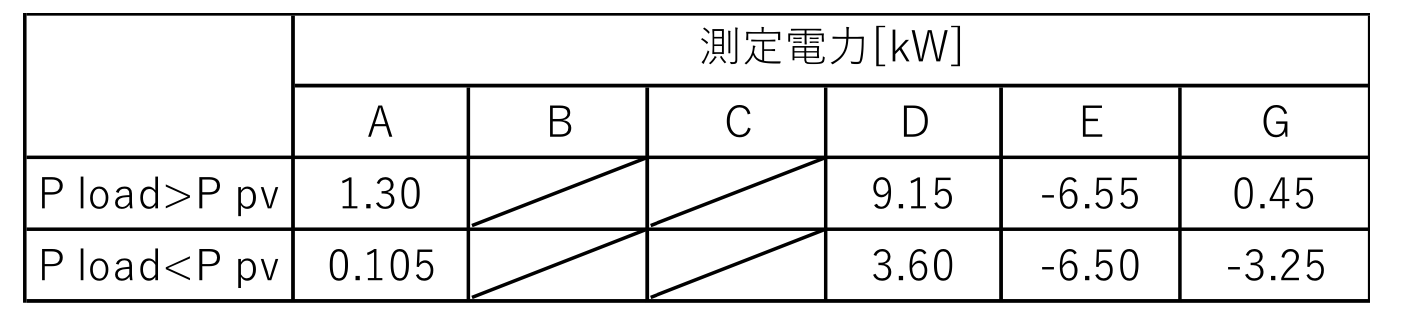
\includegraphics[width=0.8\textwidth]{./img/24-1/1.png}
                        \caption{load}
                    \end{figure}

                \subsubsection{自立モードでの実験}
                    下記の実験結果を表にまとめた。
                    自立モードでの実験では、まず需給管理装置画面の「デンリョクスケジュール」にてPtimeを0\%と設定し、需給管理装置のACスイッチのランプが消灯したことを確認する。その後、現在のPVの発電電力 \(P_{PV}\) を監視モニタより読み取り、模擬負荷用コンセントに \(P_{PV}\) よりも大きい負荷 \(P_{load}\) を接続し、A~EおよびGの電力を監視モニタより読み取り、表4に記入する。さらに、 \(P_{PV}\) よりも小さな負荷を接続した際も同様にA~EおよびGの電力を監視モニタより読み取り、表4に記入する。
                    \begin{figure}[H]
                        \centering
                        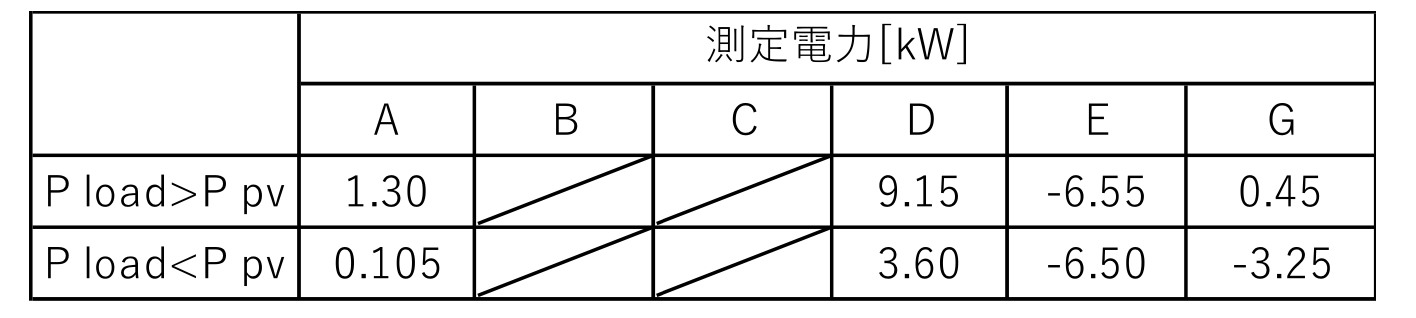
\includegraphics[width=0.8\textwidth]{./img/24-1/2.png}
                        \caption{load}
                    \end{figure}
                
                \subsubsection{系統連系モードでの実験(PV なし)}
                    下記の実験結果を表にまとめた。
                    まずMCCB 12と13を共に開放してPVを停止させ、模擬負荷用コンセントに合計5kW程度の負荷を接続する。その後、需給管理装置画面の「デンリョクスケジュール」にてPtimeを10\%とし、A~EおよびGの電力を監視モニタより読み取り、表5に記入する。次に、Ptimeを100\%とし、同様にA~EおよびGの電力を監視モニタより読み取り、表4に記入する。最後にMCCB 13を投入し、PCSを再起動させる(起動には約5分かかる)。
                    \begin{figure}[H]
                        \centering
                        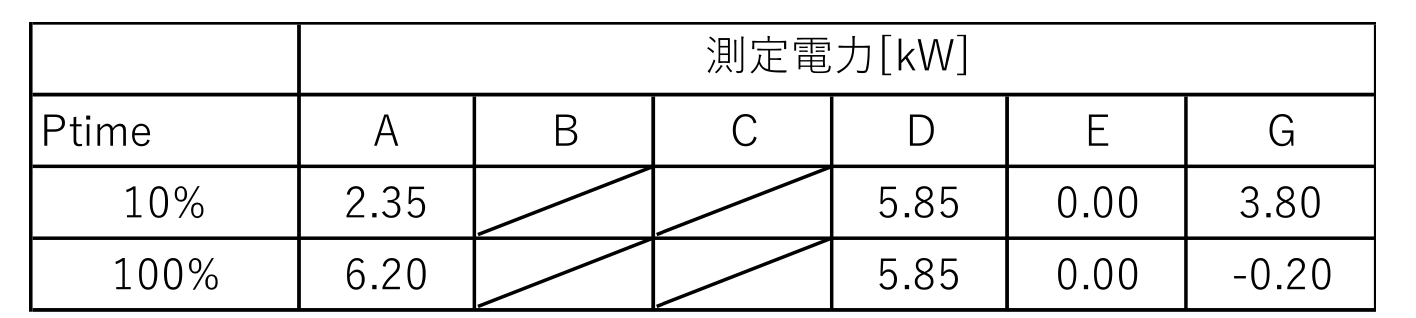
\includegraphics[width=0.8\textwidth]{./img/24-1/3.png}
                        \caption{load}
                    \end{figure}

                \subsubsection{バックアップモードでの実験(需給管理装置なし)}
                    下記の実験結果を表にまとめた。
                    まずMCCB 52Mを投入し、次にMCCB 52LとMCCB 52Cを順番に開放する。続いてMCCB 1を開放し、「需給管理装置なし」かつ「疑似的に停電状態」とする。その後、屋上前階段踊り場に設置されているPCS6の状態を確認し、再びMCCB 1を投入してから、投入直後および5分後のPCS6の様子を確認する。
                    \begin{figure}[H]
                        \centering
                        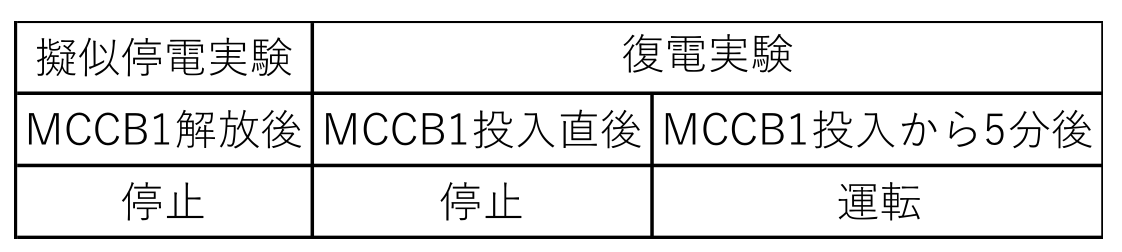
\includegraphics[width=0.8\textwidth]{./img/24-1/4.png}
                        \caption{load}
                    \end{figure}

                \subsubsection{バックアップモードでの実験(需給管理装置あり)}
                    まずMCCB 52CとMCCB 52Lを順番に投入し、その後MCCB 52Mを開放する。次にMCCB 1を開放し、「需給管理装置あり」かつ「疑似的に停電状態」とする。その後、屋上前階段踊り場に設置されているPCS6の状態を確認し、最後にMCCB 1を投入する。実験結果は開放後、動作していることが確認できた。


                \subsubsection{DC/DC コンバータの実験}
                    下記の実験結果を表にまとめた。
                    まずMCCB 12と13を共に開放してPVを停止させ、次にMCCB 4を投入してDC/DCコンバータを起動する。その後、需給管理装置画面の「デンリョクスケジュール」にてPtimeを0\%とし、ACスイッチのランプが消灯したことを確認する。次に直流模擬負荷装置の電源を入れ、矢印キーを操作して「CR-L」ランプを点滅させ、「ENTER」キーを押して抵抗動作を確定させる(「CR-L」ランプが点灯)。「PRG」ランプが点灯し、下側数字表示に現在設定されている抵抗値が表示されるので、数値設定ノブを回して抵抗値を「280 Ω 程度」に設定し、「ENTER」キーを押して下側数字表示に電流計測値を表示させる。続いて「LOAD」キーを押して負荷電流を流す。

                    DC/DCコンバータの入出力箇所で入出力の電圧・電流を計測し、表8にまとめる。入出力電流についてはクランプ電流計で10分間測定し、電圧についてはマルチテスターによりそのときの値を読み取る。5分経過後および10分経過後も同様に電圧・電流を測定する。求められた電圧・電流よりコンバータの入出力電力を算出し、入力電力と出力電力の関係からコンバータの変換効率を算出する。最後に直流模擬負荷装置とDC/DCコンバータをそれぞれ停止し、MCCB 4を開放する。

                    平均変換効率は70.62\%だった。

                    \begin{figure}[H]
                        \centering
                        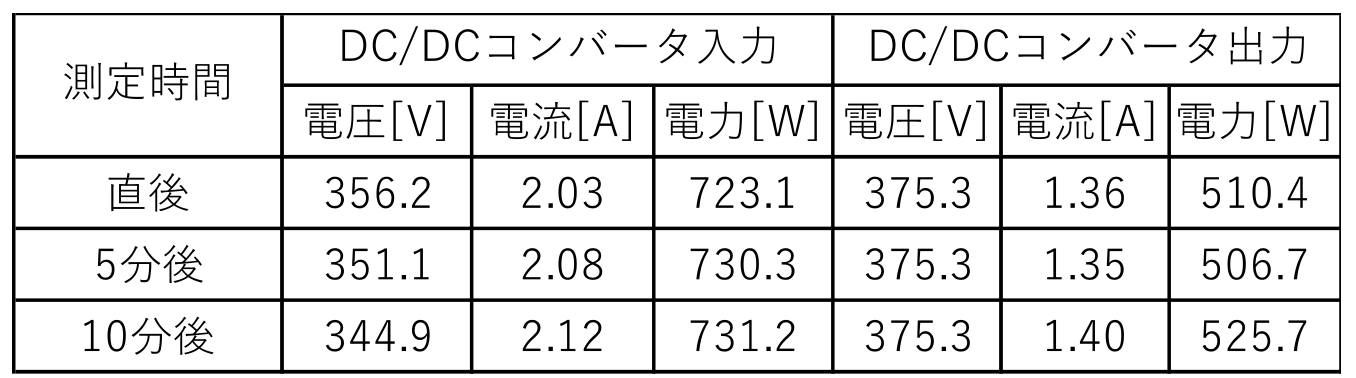
\includegraphics[width=0.8\textwidth]{./img/24-1/5.png}
                        \caption{load}
                    \end{figure}


            \subsubsection{まとめ}
                PCS(Power Conditioning System)は停電時に自動的に遮断されますが、その理由は安全確保とシステム保護にあります。停電時にPCSが稼働し続けると、系統側に送電される可能性があり、電力会社の作業員にとって危険です。また、突然の停電によってシステムに過負荷や過電流が生じる可能性があるため、PCSは自動的に遮断されて機器を保護します。

                PCSが投入された後すぐに復電しない理由としては、自己診断や系統電圧や周波数への同期手順が時間を要すること、内部のキャパシタの充電が必要なことが挙げられます。

                蓄電池から直流負荷に電力を供給する際にDC/DCコンバータが必要となる理由は、電圧変換、効率向上、負荷適合性にあります。蓄電池の出力電圧は一定ではなく、充放電の状態に応じて変動するため、直流負荷が必要とする電圧に適合させるためにDC/DCコンバータで安定した電圧を供給する必要があります。また、DC/DCコンバータを使用することでエネルギー効率を高め、各種直流負荷の要件に合わせて必要な電圧や電流を供給することができます。

                日本ではスマートグリッドの導入が進んでおり、再生可能エネルギーの普及に伴い、電力系統の安定化と効率化を図るための技術が開発・実装されています。再生可能エネルギーの統合やエネルギーマネジメントシステム(EMS)の普及が進んでいます。スマートコミュニティでは、地域全体のエネルギー管理と効率化を目指し、地域エネルギーマネジメントやスマートホームの普及が進んでいます。これらの取り組みにより、日本ではエネルギーの効率的な利用と環境負荷の低減が図られています。


\end{document}
